\chapter{The CMS Experiment and the LHC}
\label{ch:cms}
The Compact Muon Solenoid (CMS) detector is a multi-purpose detector
conceived to study proton-proton (and lead-lead) collisions produced
by the Large Hadron Collider (LHC) at CERN~\cite{Adolphi:2008zzk}.

The ultimate goals of the LHC physics programme are to elucidate the nature of
electroweak symmetry breaking and search for evidence of new symmetries, new
forces, or new constituents of matter that could pave the way toward a
unified theory beyond the standard model. There are several detector
and readout requirements for CMS to meet these goals:
\begin{itemize}
\item Good muon identification and momentum resolution over a wide
  range of momenta, good dimuon mass resolution ($\approx 1\%$ at 100
  \GeV), and the ability to unambiguously determine the charge of muons
  with $p<1 \TeV$. See Sec.~\ref{sec:muon};
\item Good charged particle momentum resolution and reconstruction
efficiency in the inner tracker. Efficient triggering and offline
identification of $\Pgt$ leptons and \PQb-jets, requiring pixel
detectors close to the interaction region. See Sec.~\ref{sec:tracker};
\item Good electromagnetic energy resolution, good diphoton and
  dielecron mass resolution ($\approx 1\%$ at 100 \GeV), wide
  geometric coverage, $\pi^0$ rejection, and efficient photon and
  lepton isolation at high luminosities. See Sec.~\ref{sec:ecal};
\item Good missing-transverse-energy and dijet-mass resolution,
  requiring hadron calorimeters with hermetic geometric coverage and
  fine lateral segmentation. See Sec.~\ref{sec:hcal};
\item Fast online event selection process (\emph{trigger}) to reduce the rate from $10^9$ inelastic collision
  events per second to $\lesssim1000$ events per second for storage
  and subsequent analysis. See Sec.~\ref{sec:trigger};
\item Infrastructure for the alignment and calibration of the detector. See Sec.~\ref{sec:alca}.
\end{itemize}
The design of CMS, pictured in Fig.~\ref{fig:CMSperspective} and detailed
in the following sections, meets these requirements. Each detector subsystem is
integral to the performance of CMS as a whole and is specialized to a
particular class of particles, as seen in Fig.~\ref{fig:CMSslice}: the silicon
tracker measures the tracks of charged particles, the electromagnetic
calorimeter measures the energy of electrons and photons, the hadron calorimeter measures the
energy of charged and neutral hadrons, the
superconducting solenoid bends the tracks of charged particles to
allow for a precise momentum measurement, and the muon detectors
identify and measure the momentum of muons.

%The central feature of the CMS detector is a
%superconducting solenoid of 6\unit{m} internal diameter, providing a
%magnetic field of 3.8\unit{T}. Within the superconducting solenoid
%volume are a silicon pixel and a silicon strip tracker, a
%lead-tungstate crystal electromagnetic calorimeter, and a
%brass/scintillator hadron calorimeter, each composed of a barrel and
%two endcap sections. Muons are measured in gas-ionization detectors
%embedded in the magnet steel flux-return yoke outside the
%solenoid. Extensive forward calorimetry complements the coverage
%provided by the barrel and endcap detectors. Jets and leptons are
%econstructed within the pseudorapidity region $\abs{\eta}<3$, covered by the
%electromagnetic and hadron calorimeters. Muons are reconstructed with
%$\abs{\eta}<2.4$. Events are selected by a two-level trigger system. The first level (L1) is based on a hardware
%filter, followed by a software-based high level trigger (HLT). 

\begin{figure}
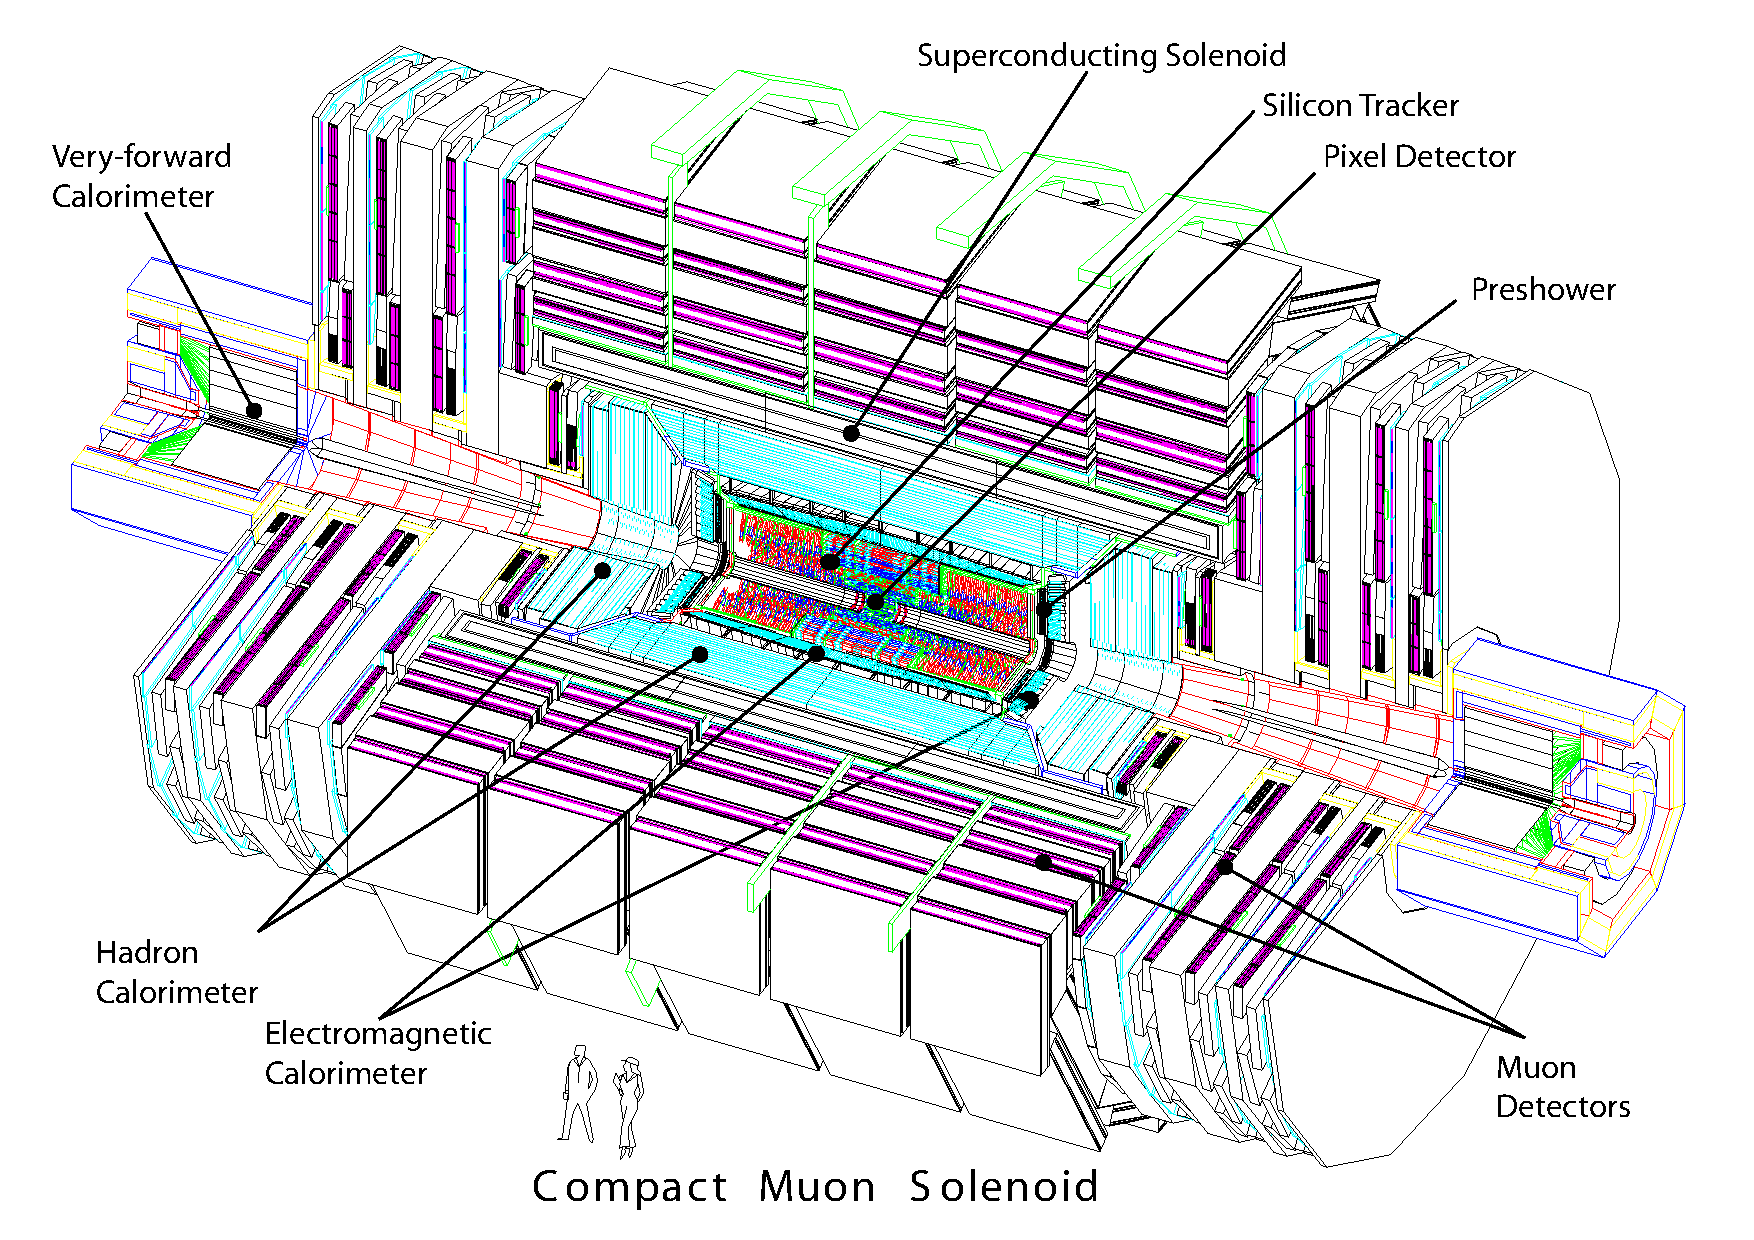
\includegraphics[width=.9\textwidth]{figs/cms/Figure_001-002.pdf}
\caption{Perspective view of the CMS detector.\label{fig:CMSperspective}}
\end{figure}

\begin{figure}
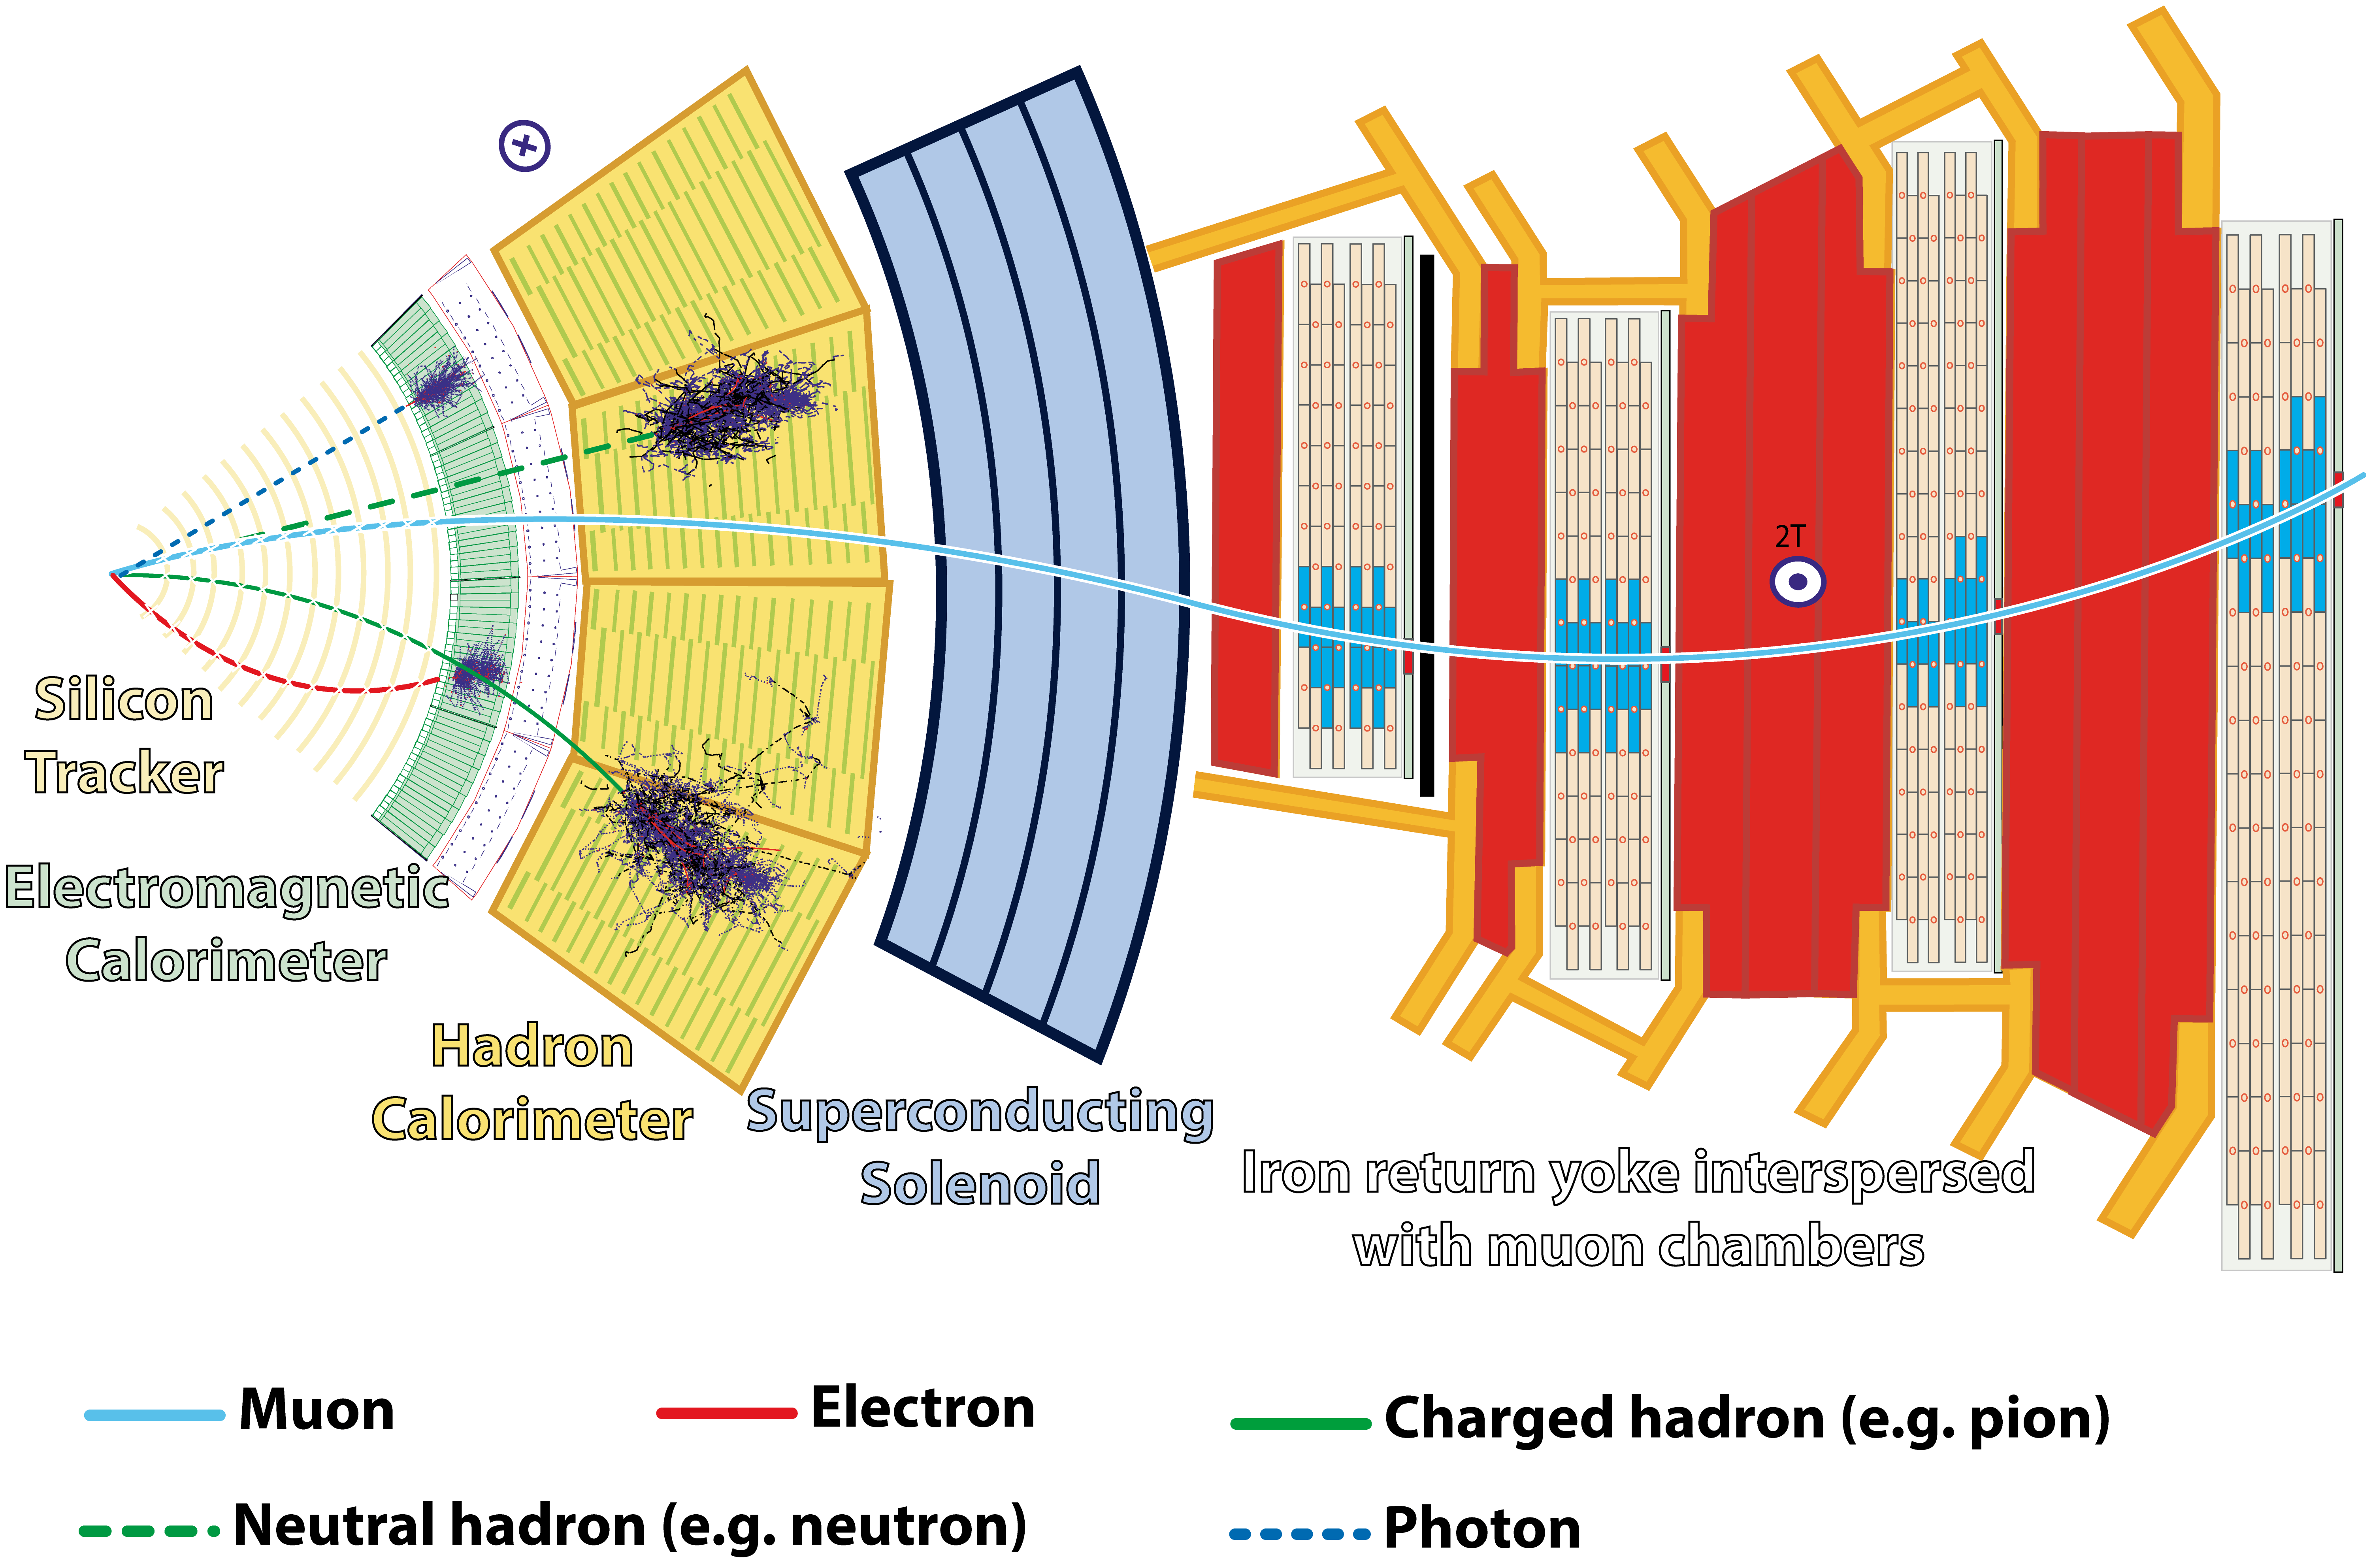
\includegraphics[width=.9\textwidth]{figs/cms/CMSslice_whiteBackground.png}
\caption{A slice of the CMS detector.\label{fig:CMSslice}}
\end{figure}

\section{Large Hadron Collider}
The Large Hadron Collider (LHC) is a 27\unit{km} two-ring superconducting
proton accelerator and collider located at CERN, spanning the border between
France and Switzerland.  At design specifications, the LHC will collide
protons at a center-of-mass energy of 14\TeV and instantaneous
luminosity $10^{34} \unit{cm}^{-2} \unit{s}^{-1}$.
\begin{table*}
\centering
 \caption{Comparison between LHC design parameters and achieved
   parameters in 2012 and 2015.
 \label{tab:LHCparameters}}
\resizebox{\textwidth}{!}{
\begin{tabular}{|l|c|c|c|c|}
\hline 
Parameter & Unit & \textbf{Design} & \textbf{Acheived (2012)} & \textbf{Acheived (2015)} \\\hline
\multicolumn{5}{|c|}{\textbf{Beam Data}}\\\hline
Proton energy & [GeV] & 7000 & 4000 & 6500 \\\hline
Relativistic gamma factor $\gamma_r$ & & 7461 & 4263 & 6928 \\\hline
Number of particles per bunch $N_b$ & & $1.15\times10^{11}$ &
                                                        $1.6-1.7\times10^{11}$ & $1.15\times10^{11}$ \\\hline
Number of bunches $n_b$ & & 2808 & 1374 & 2244 \\\hline
Bunch spacing & [ns] & 25 & 50 & 25 \\\hline
%Longitudinal emittance ($4\sigma$) & [eV s] & 2.5 & & \\\hline
Transverse normalized emittance $\varepsilon_n$& [$\mu$m rad] & 3.75
                                   &2.5& $\geq2.7$\\\hline
Circulating beam current & [A] & 0.582 & 0.369&\\\hline
Stored energy per beam & [MJ] & 362 & 140 &\\\hline
\multicolumn{5}{|c|}{\textbf{Peak Luminosity Related Data}}\\\hline
$\beta^{\ast}$ at IP1 and IP5 & [m] &0.55 & 0.6 & 0.8 \\\hline
RMS bunch length $\sigma_z$& [cm] & 7.55 & $\geq 9$ &\\\hline
RMS beam size at IP1 and IP5 $\sigma^{\ast}$ & [$\mu$m] & 16.7 & 19 &\\\hline 
Half crossing angle at IP1 and IP5 $\theta_c/2$& [$\mu$rad] & $\pm142.5$ &
                                                               $\pm145.0$ & $\pm145.0$\\\hline
Geometric luminosity reduction factor $F$ & &0.836 & &\\\hline
Peak luminosity in IP1 and IP5 & [cm$^{-1}$s$^{-1}$] &
                                                       $1.0\times10^{34}$ & $7.7\times10^{33}$ & $5.2\times10^{33}$ \\\hline
Max. mean number of events per bunch crossing& & 19 & 40 & 17 \\\hline
\end{tabular}
}
\end{table*}

The LHC is the pinnacle of the accelerator
complex at CERN, pictured in Fig.~\ref{fig:LHCComplex}.  To accelerate
protons to a beam energy of 6.5\TeV in the LHC, a chain of smaller
accelerators are needed. Starting from bottle of hydrogen gas,
electrons are stripped from the hydrogen atoms by an electric field
and the resulting protons enter the Linac 2, which accelerates the
protons to 50\MeV. Subsequently, the Proton Synchrotron Booster (PSB), Proton Synchrotron (PS), and the
Super Proton Synchrotron (SPS) accelerate the protons to 1.4\GeV, 25\GeV, and 450\GeV, respectively, before they are finally injected
into the two LHC rings as counter-rotating beams.

\begin{figure}
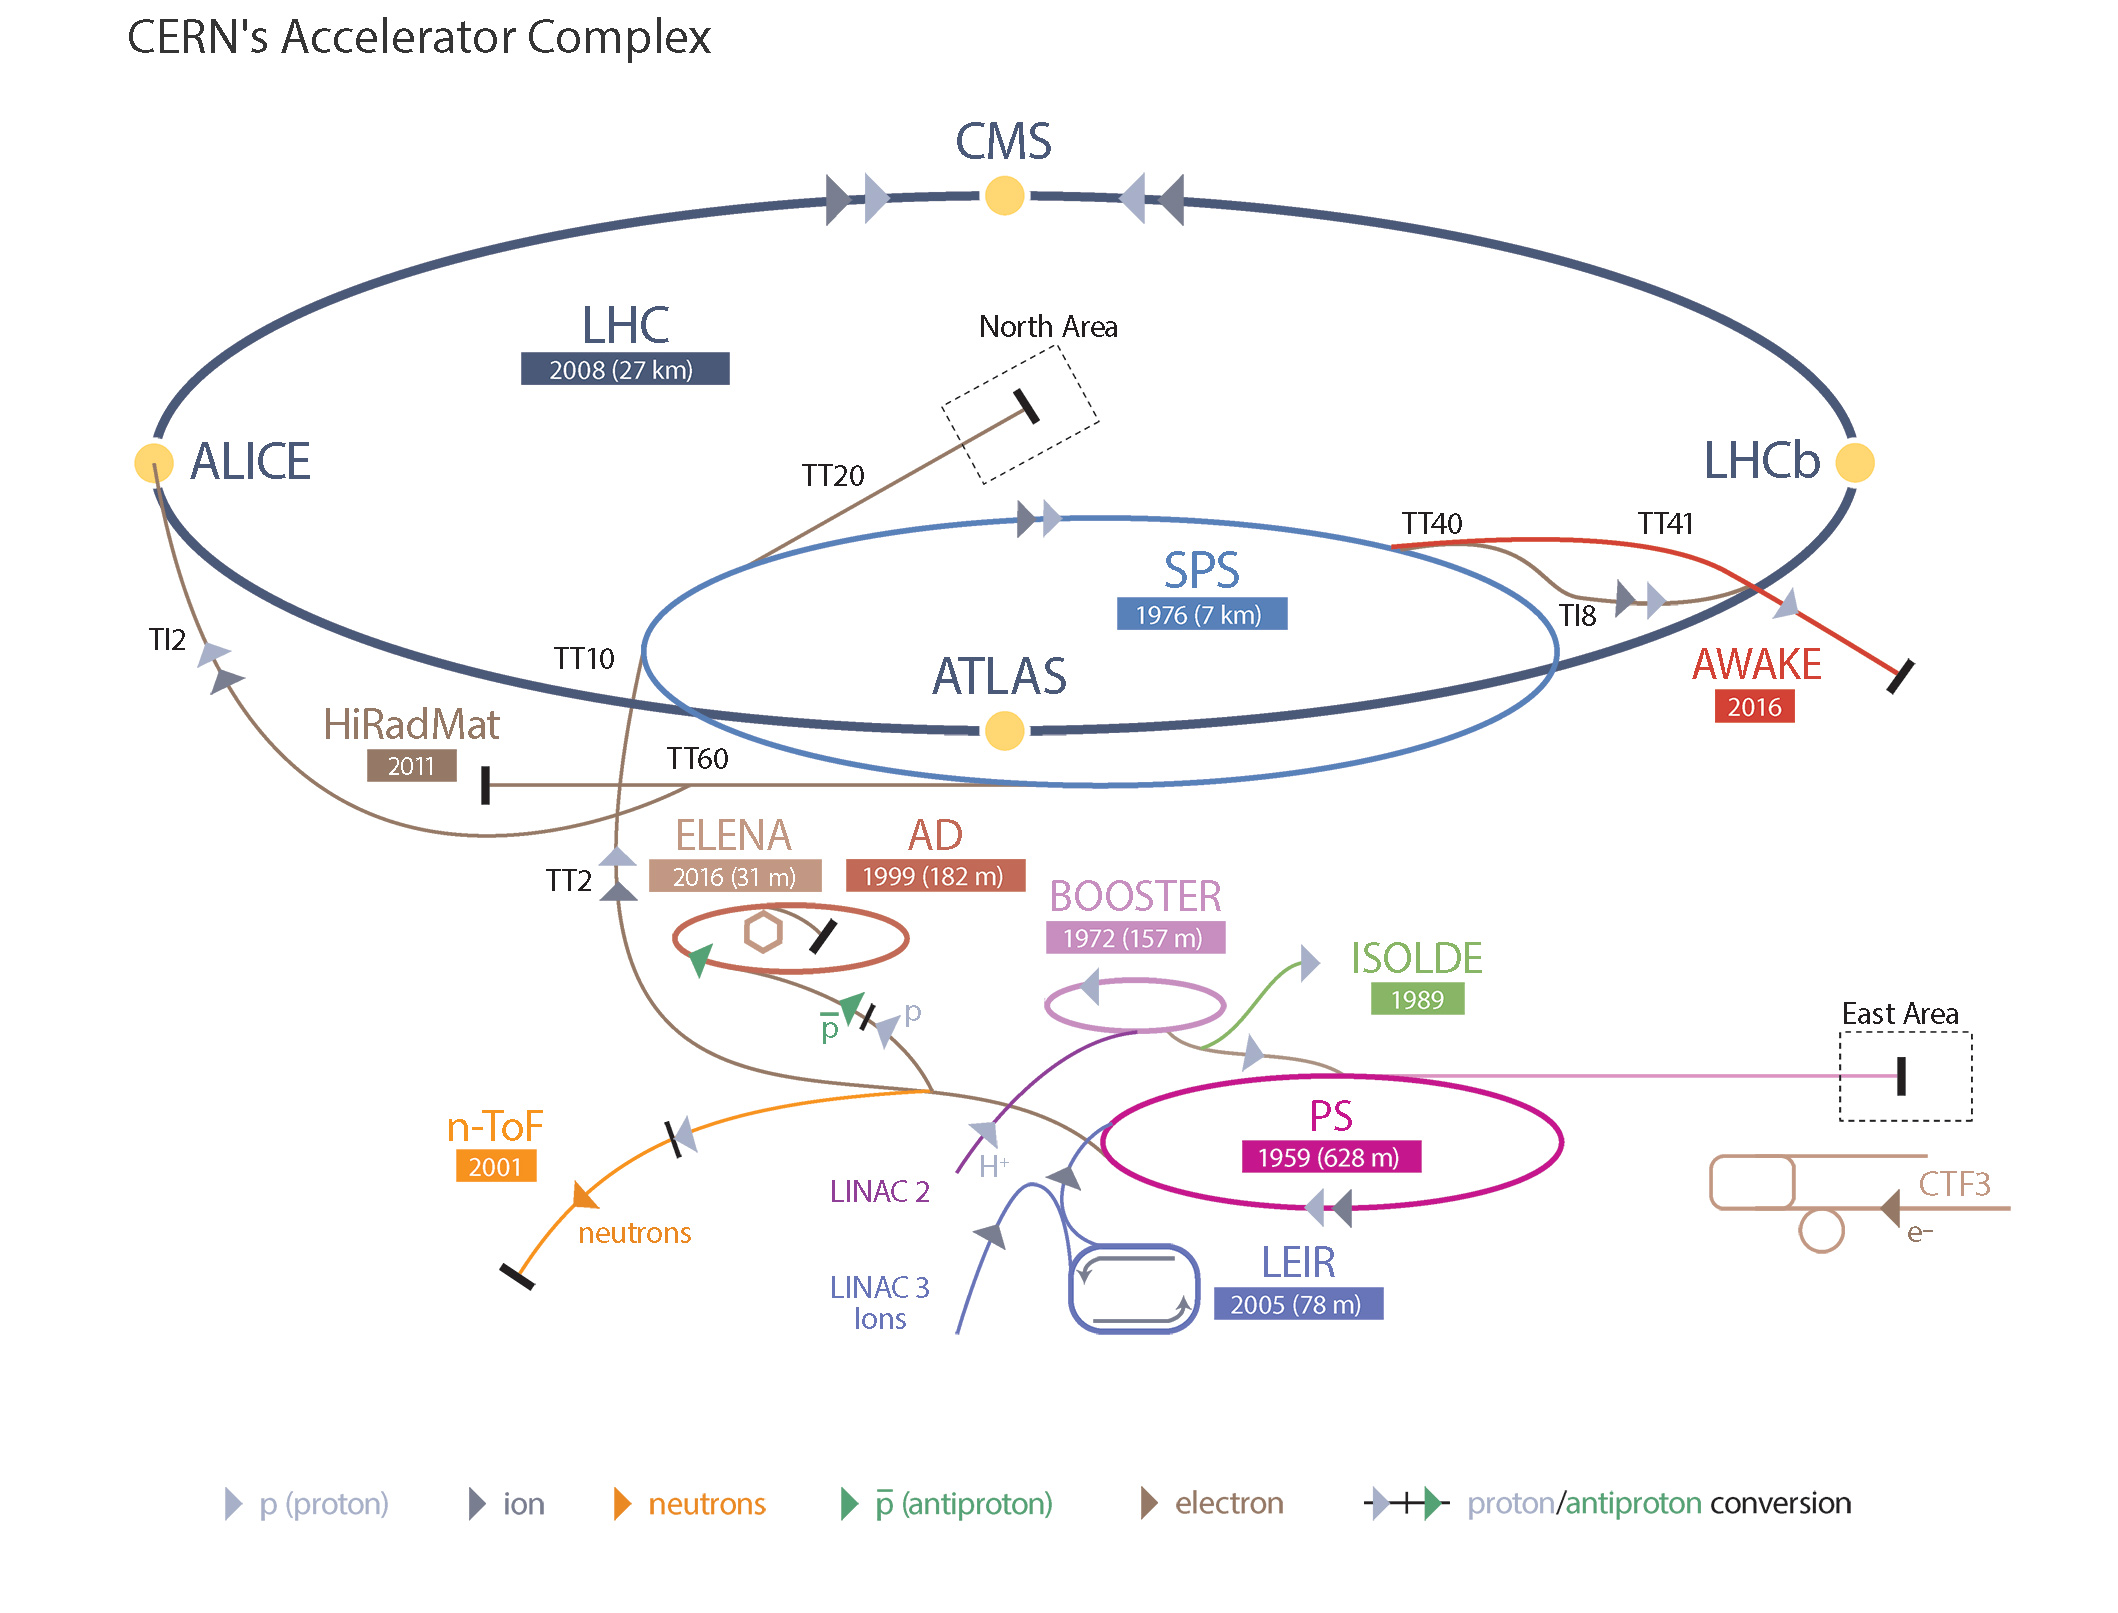
\includegraphics[width=.9\textwidth]{figs/cms/LHC_default.jpg}
\caption{CERN's accelerator complex.\label{fig:LHCComplex}}
\end{figure}

One of the main features influencing the design of the LHC is the re-use of the
existing 26.7\unit{km} tunnel from the Large Electron Positron collider (LEP), which is
comprised of eight crossing points (or arcs) and eight straight sections for
RF cavities. The tunnel in the arc sections has an internal diameter of 3.7\unit{m}. Due to the limited available space, two completely separate
proton rings would be extremely difficult to install.  magnets
would be  difficult to fit in which makes the twin-bore magnet design proposed by John
Blewett in 1971~\cite{Blewett:1068131} ideal due to its
``two-in-one'' use of the limited space. A cross-section of the main superconducting
dipole magnet is shown in \ref{fig:LHCDipole}.

\begin{figure}
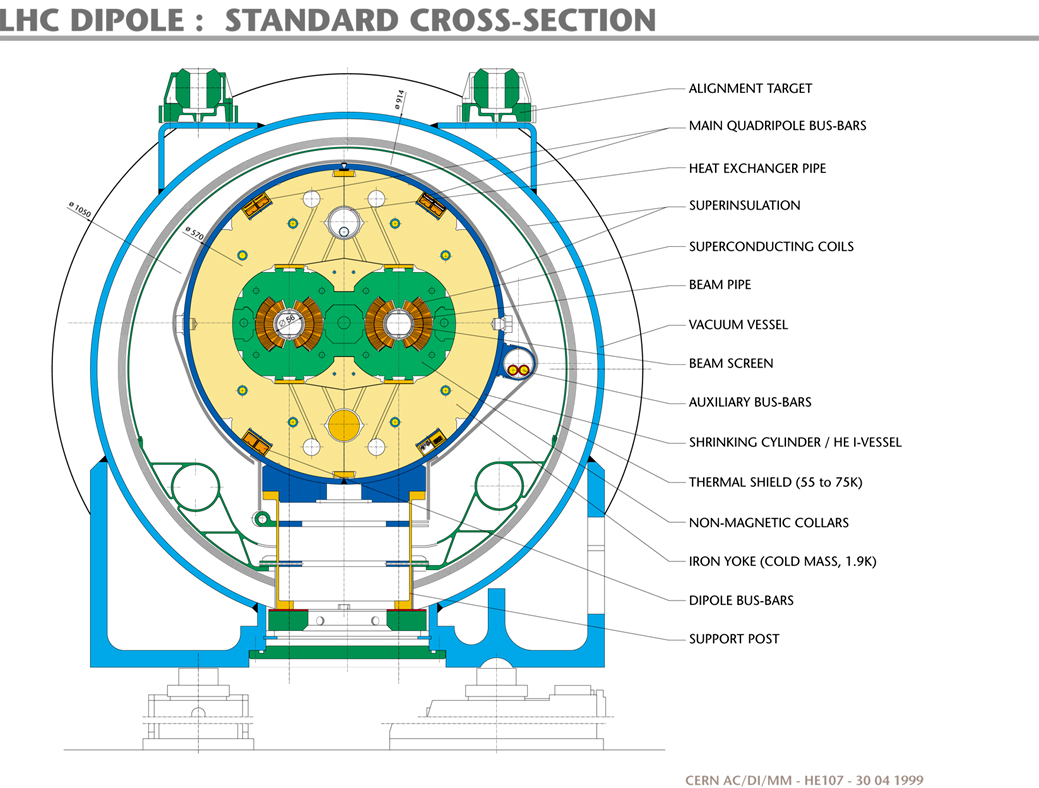
\includegraphics[width=.9\textwidth,clip=true,viewport=0 20 680 550]{figs/cms/lhc-pho-1999-172.jpg}
\caption{Cross-section of the LHC dipole magnet.\label{fig:LHCDipole}}
\end{figure}

The observed number of events $N_{\mathrm{exp}}$ is the product of the cross
section of interest $\sigma_{\mathrm{exp}}$ and the time integral of
the instantaneous luminosity,
\begin{equation}
N_{\mathrm{exp}}  =\sigma_{\mathrm{exp}}\int \mathscr{L}(t)dt ~.
\end{equation}
The instantaneous luminosity depends on the beam parameters and
can be written for a Gaussian beam distribution as~\cite{LHCMachine}:
\begin{equation}
\mathscr{L} =
\frac{N_b^2n_bf_{\mathrm{rev}}\gamma_r}{4\pi\varepsilon_n\beta^{\ast}}F~,
\label{eqn:instlumi}
\end{equation}
where $N_b$ is the number of particles per bunch, $n_b$ the number
of bunches per beam, $f_{\mathrm{rev}}$ the revolution frequency,
$\gamma_r$ the relativistic gamma factor, $\varepsilon_n$ the
normalized transverse beam emittance, $\beta^{\ast}$ the beta function
at the collision point, and $F$ the geometric luminosity reduction
factor due to the crossing angle at the interaction point (IP):
\begin{equation}
F=\left(1+\left(\frac{\theta_c\sigma_z}{2\sigma^{\ast}}\right)^2\right)^{-1/2}~,
\label{eqn:F}
\end{equation}
where $\theta_c$ is the full crossing angle, $\sigma_z$ is the RMS
bunch length, and $\sigma^{\ast}$ is the RMS bunch size.


\section{Superconducting Solenoid}
\label{sec:magnet}
The central feature of the CMS detector is a
superconducting solenoid providing a uniform axial
magnetic field of 3.8\unit{T}  over a magnetic length of 12.5 \unit{m}
and a free-bore radius of 3.15 \unit{m}. The large bending power ($11.4$ \unit{T}\unit{m}) of the
superconducting magnet permits a precise measurement of the momentum
of high-energy charged particles. The return field is large enough to
saturate $1.5$ \unit{m} of iron, allowing four \emph{muon stations} to be
integrated to ensure robustness and full geometric coverage. The bore
of the magnet coil is large enough to accommodate the inner tracker
and the calorimetry inside, thereby minimizing the amount of material
in front of the calorimeters.

\section{Silicon Tracker}
\label{sec:tracker}
The first layer of the detector encountered by outgoing particles from the
collisions is the tracker, composed of a small silicon pixel
surrounded by a large silicon strip tracker~\cite{Chatrchyan:2014fea}. Both tracker subdetectors are
cylinder-shaped and occupy a total $5.8$ \unit{m} in length and $2.5$
\unit{m} in diameter. The pixel detector barrel (endcaps) comprises three (two) layers of pixel
detectors, providing three-dimensional position measurements of the
hits arising from the interaction of charged particles with its
sensors. The hit position resolution is approximately $10$ $\mu$m in
the transverse coordinate and $20–40$ $\mu$m in the longitudinal
coordinate, while the third coordinate is given by the sensor plane
position. In total, its $1440$ modules cover an area of about 1
m$^{2}$ and have $66$ million pixels.

%The pixel detector consists of cylindrical barrel layers at radii of 4.4, 7.3 and 10.2 cm, and two pairs of endcap disks at z = ±34.5 and ±46.5 cm. It provides three-dimensional (3-D) position measurements of the hits arising from the interaction of charged particles with its sensors.

Surrounding this is the silicon strip tracker. The silicon detector
barrel (endcaps) has ten (twelve) layers of micro-strip detectors. In
total, the with
$15,148$ silicon modules, which cover an active area of about $198$
m$^2$ and have $9.3$ million strips. 

%It is composed of four subsystems. The Tracker Inner Barrel (TIB) and Disks
%(TID) cover r < 55 cm and |z| < 118 cm, and are composed of four
%barrel layers, supplemented by three disks at each end. These provide
%position measurements in rφ with a resolution of approximately 13–38
%μm. The Tracker Outer Barrel (TOB) covers r > 55 cm and |z| < 118 cm
%and consists of six barrel layers providing position measurements in
%rφ with a resolution of approximately 18–47 μm. The Tracker EndCaps
%(TEC) cover the region 124 < |z| < 282 cm. Each TEC is composed of
%nine disks, each containing up to seven concentric rings of silicon
%strip modules, yielding a range of resolutions similar to that of the
%TOB.

The fine granularity of the two tracker subdetectors offers separation of closely-spaced particle
trajectories in energetic jets. Fig.~\ref{fig:tracker} shows a
schemetic layout of the tracker in the $r-z$ plane and
the material budget of the CMS tracker, both in units of radiation
lengths and nuclear interaction lengths, as estimated from
simulation. 
%The simulation describes the tracker material budget with
%an accuracy better than 10\%, as was established by measuring the
%distribution of reconstructed nuclear interactions and photon
%conversions in the tracker.

\begin{figure}
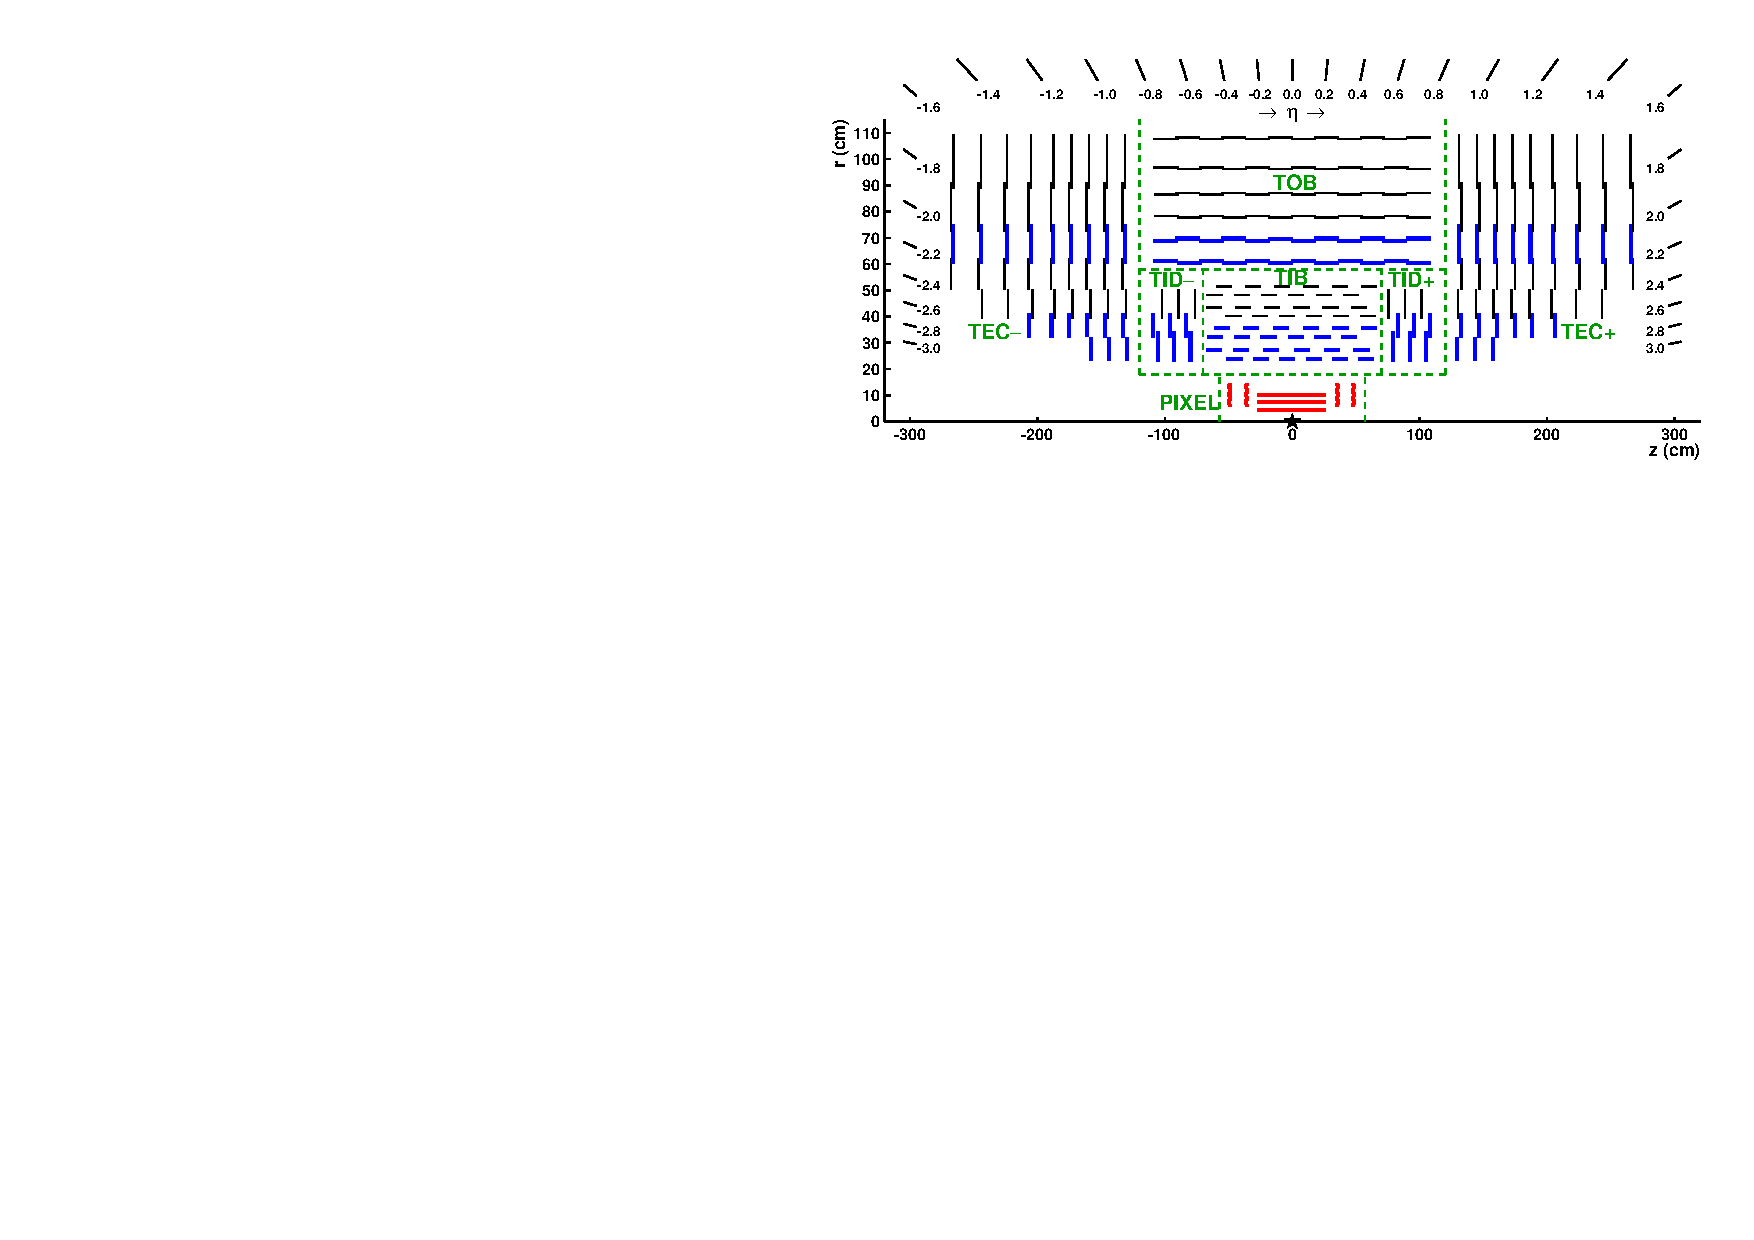
\includegraphics[width=.9\textwidth]{figs/cms/TrackerLayoutNew.pdf}\\
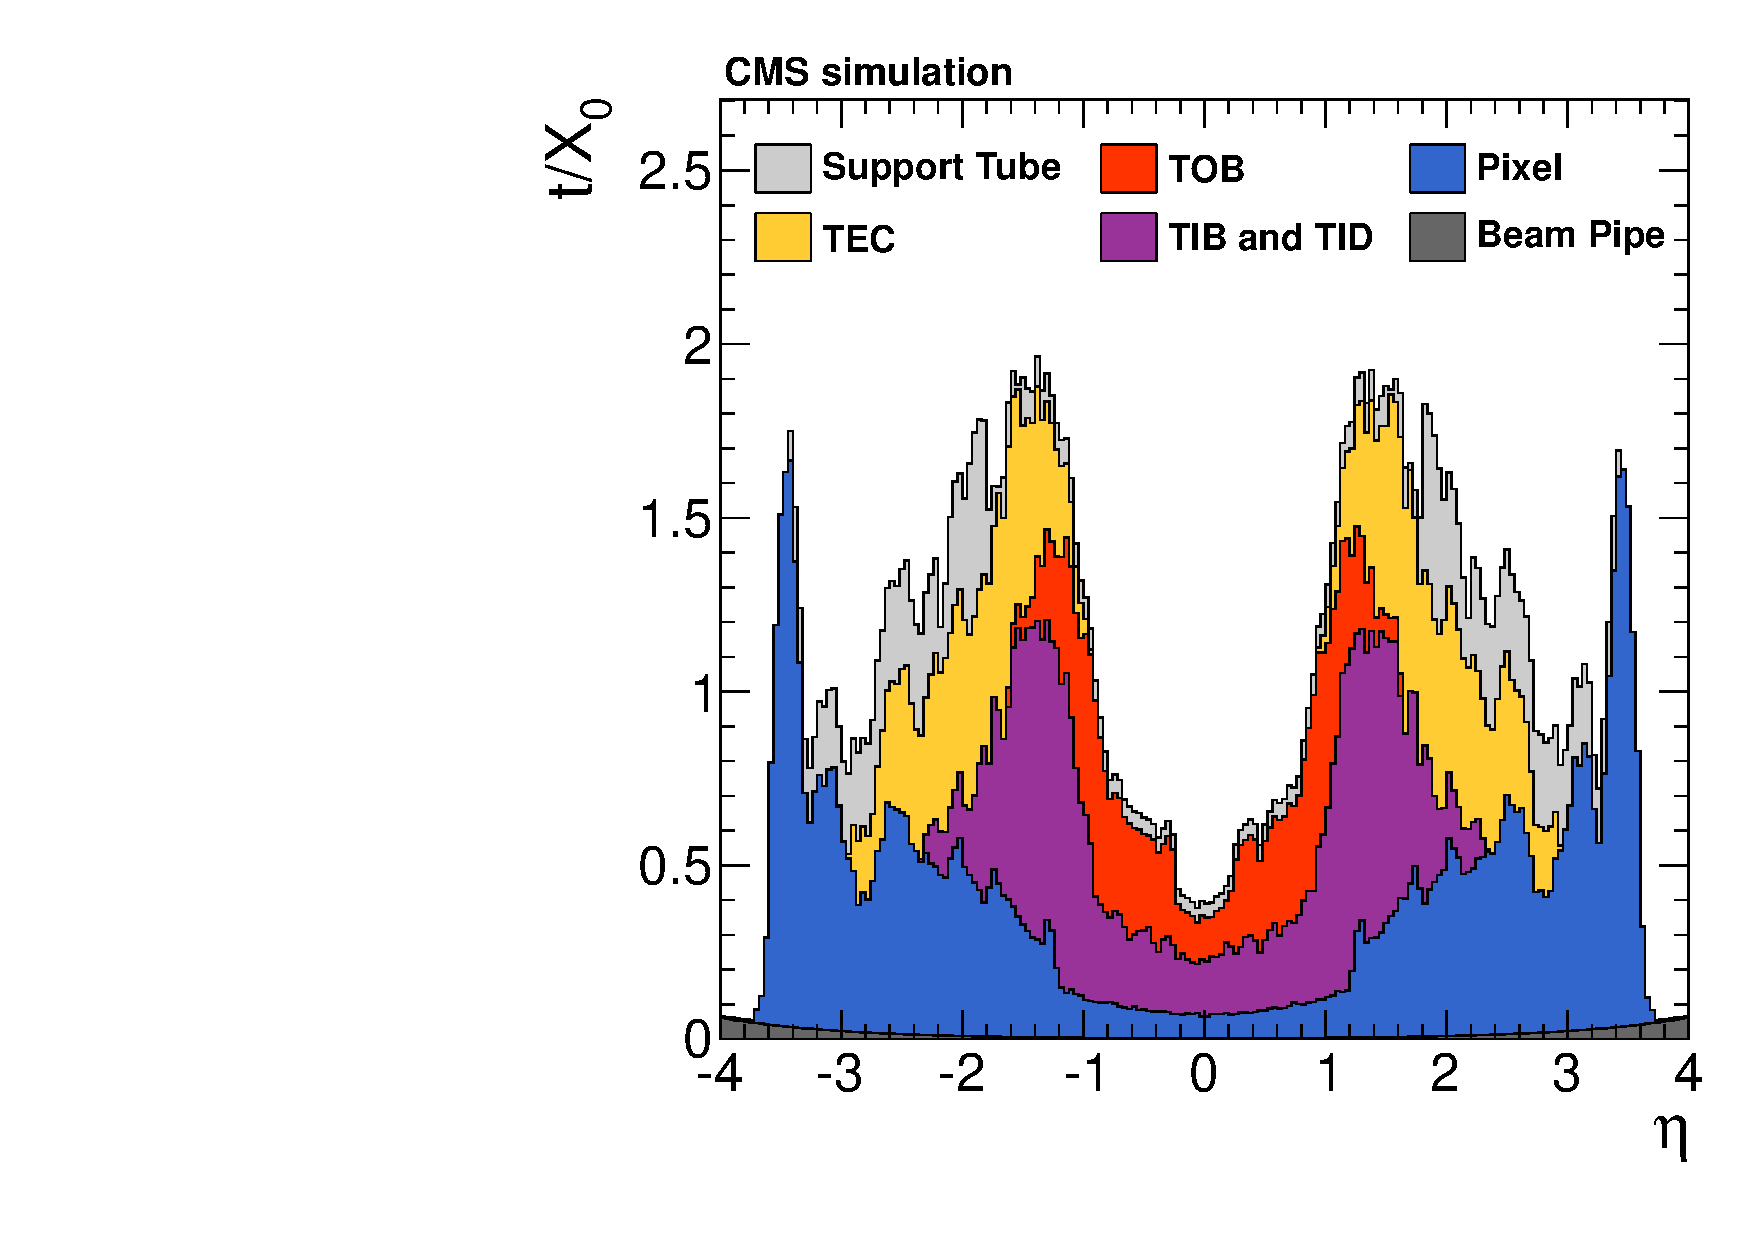
\includegraphics[width=.45\textwidth]{figs/cms/MaterialBudget_RadLengths.pdf}
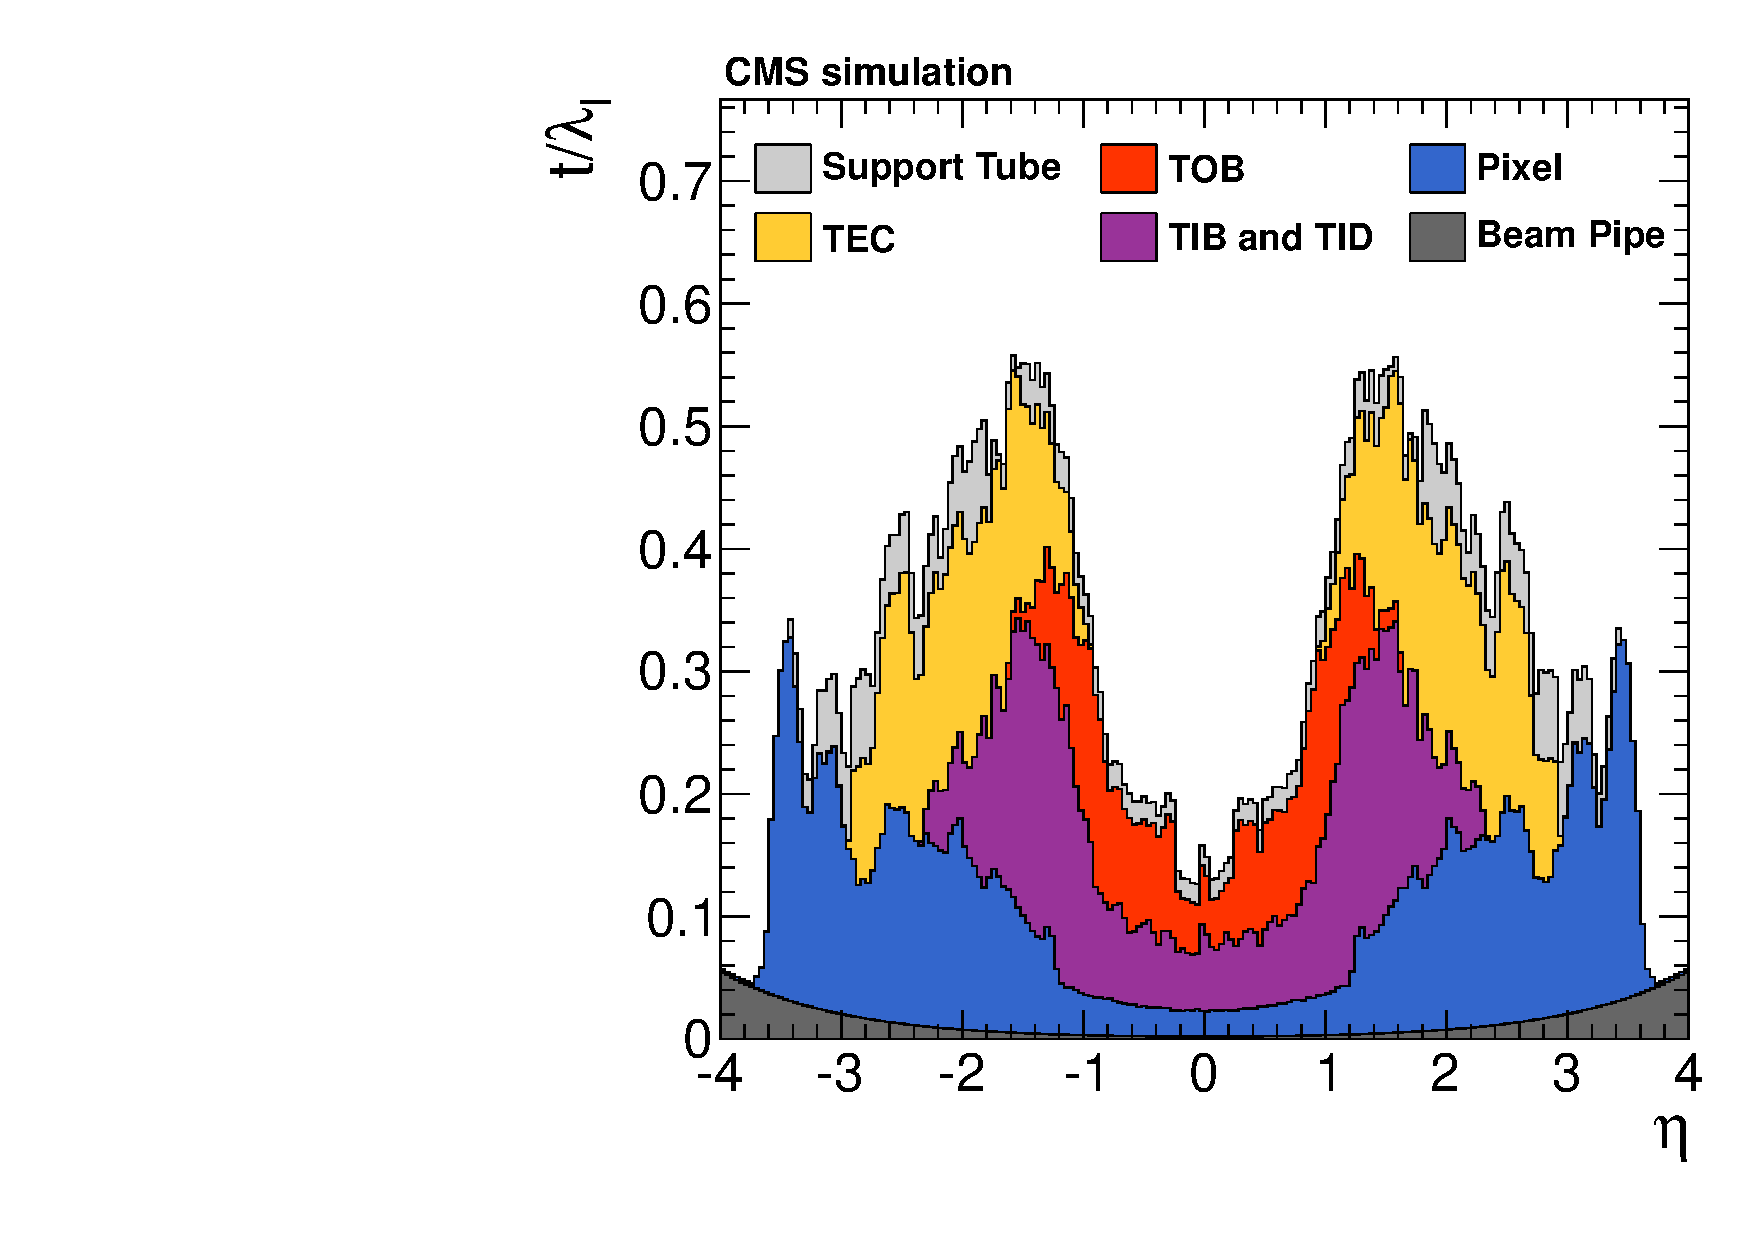
\includegraphics[width=.45\textwidth]{figs/cms/MaterialBudget_InteractionLengths.pdf}
\caption{ (Top) Schematic cross section through the CMS tracker in the $r-z$
  plane. (Bottom) Total thickness $t$ of the tracker material
  traversed by a particle produced at the nominal interaction point,
  as a function of pseudorapidity η, expressed in units of radiation
  length $X_0$ (left) and nuclear interaction length $\lambda_I$
  (right). 
%In this view, the tracker is symmetric about the horizontal
%  line $r = 0$, so only the top half is shown. The center of the
%  tracker, corresponding to the approximate position of the pp
%  collision point, is indicated by a star. Green dashed lines help the
%  reader understand which modules belong to each of the named tracker
%  subsystems. Strip tracker modules that provide 2D hits are shown by
%  thin, black lines, while those permitting the reconstruction of hit
%  positions in 3D are shown by thick, blue lines. The latter actually
%  each consist of two back-to-back strip modules, in which one module
%  is rotated through a `stereo' angle. The pixel modules, shown by the
%  red lines, also provide 3D hits. Within a given layer, each module
%  is shifted slightly in $r$ or $z$ with respect to its neighbouring
%  modules, which allows them to overlap, thereby avoiding gaps in the
%  acceptance.
\label{fig:tracker}}
\end{figure}


\section{Electromagnetic Calorimeter}
\label{sec:ecal}

Within the superconducting solenoid volume and just outside of the
tracker, lies the electromagnetic
calorimeter (ECAL), a hermetic homogenous calorimeter composed of
lead-tungstate (PbWO$_{4}$)
scintillating crystals covering pseudorapidities up to
$\abs{\eta}<1.479$ with the barrel detector, and from $1.479$ to $3.0$
with the two endcap disks.

The ECAL barrel energy resolution for electrons is measured in
an electron test beam to be~\cite{Adzic:2007mi,Chatrchyan:2013dga},
\begin{align}
\frac{\sigma_E}{E} &= \frac{S}{\sqrt E (\GeV)} \oplus \frac{N}{E (\GeV)} \oplus C \\
&= \frac{2.8\%}{\sqrt E (\GeV)} \oplus \frac{12\%}{E (\GeV)} \oplus 0.3\%
\end{align}
%\\&= \frac{7\%}{\sqrt E (\GeV)} \oplus \frac{35\%}{E (\GeV)} \oplus 0.7\%
where the three contributions are the stochastic, noise, and constant terms.

A finer-grained detector, known as the preshower, is installed in
front of each endcap disks. It consists of two layers, each comprising
a lead radiator followed by a plane of silicon strip sensors, with a pitch of $1.9$ \unit{mm}.
%The two lead radiators represent approximately two and one radiation lengths,
%respectively. The two planes of silicon sensors have orthogonal strips
%with a pitch of $1.9$ \unit{mm}. When either a photon or an electron
%passes through the lead, it initiates an electromagnetic shower. The
%granularity of the detector and the small radius of the initiating
%shower provide an accurate measurement of the shower
%position. 
Originally, the aim of the preshower superior granularity
was twofold: (i) resolve the photons from $\pi^0$ decays as to discriminate
them from prompt photons and (ii) signal the presence of a
photon/electron in the ECAL by requiring an associated signal in the
preshower. However, the high probability for photons to convert and for
electrons to radiate, and the large number of $\pi^0$s produced by hadron
interactions in the tracker material generates parasitic signals in
the preshower, thereby substantially affecting its identification and
separation capabilities.

\section{Hadron Calorimeter}
\label{sec:hcal}

The ECAL is surrounded by a hermetic sampling hadron
calorimeter (HCAL) consisting of several layers of brass absorber and plastic scintillator
tiles interleaved. A barrel detector ($\abs{\eta}<1.3$) and two endcap
disks ($1.3<\abs{\eta}<3.0$) provide pseudorapidity coverage up to
$3.0$. The scintillation light is converted by wavelength-shifting (WLS) fibers
embedded in the scintillator tiles and channeled to photodetectors via
clear fibers. This light is detected by photodetectors (hybrid
photodiodes, or HPDs) that can provide gain and operate in high axial
magnetic fields. This central calorimetry is complemented by a
tail-catcher in the barrel region (HO) ensuring that hadronic
showers are sampled with nearly 11 hadronic interaction
lengths.

The HCAL is read out in individual towers with a cross section of
$\Delta\eta\times\Delta\phi = 0.087 \times 0.087$ for $\abs{\eta}<1.6$
and $0.17\times 0.17$ at larger pseudorapidities. The HCAL energy resolution is measured in a pion test beam to
be~\cite{Abdullin:2009zz}
\begin{align}
\frac{\sigma_E}{E} &= \frac{110\%}{\sqrt E (\GeV)} \oplus 9\%~.
\end{align}

Coverage up to a pseudorapidity of $5.0$ is provided by a forward
hadron calorimeter (HF) situated at 11 \unit{m} from the interaction
point.The HF consists of a steel absorber composed of grooved
plates. Radiation-hard quartz fibers are inserted in the grooves along
the beam direction. The \v{C}erenkov light emitted in the
quartz fibers is detected by photomultipliers. The forward
calorimeters ensure full geometric coverage for the measurement of the
transverse energy in the event. 

\section{Muon System}
\label{sec:muon}

Muons are measured in gas-ionization detectors embedded in the magnet
steel flux-return yoke outside the solenoid. Each muon
station consists of several layers of aluminium drift tubes (DT) in
the barrel region and cathode strip chambers (CSC) in the endcap
region, complemented by resistive plate chambers (RPC). 

\section{Particle Flow Reconstruction}
\label{sec:pf}


\section {Level-1 and High Level Trigger}
\label{sec:trigger}

\section{Alignment and Calibration}
\label{sec:alca}

\begin{figure}
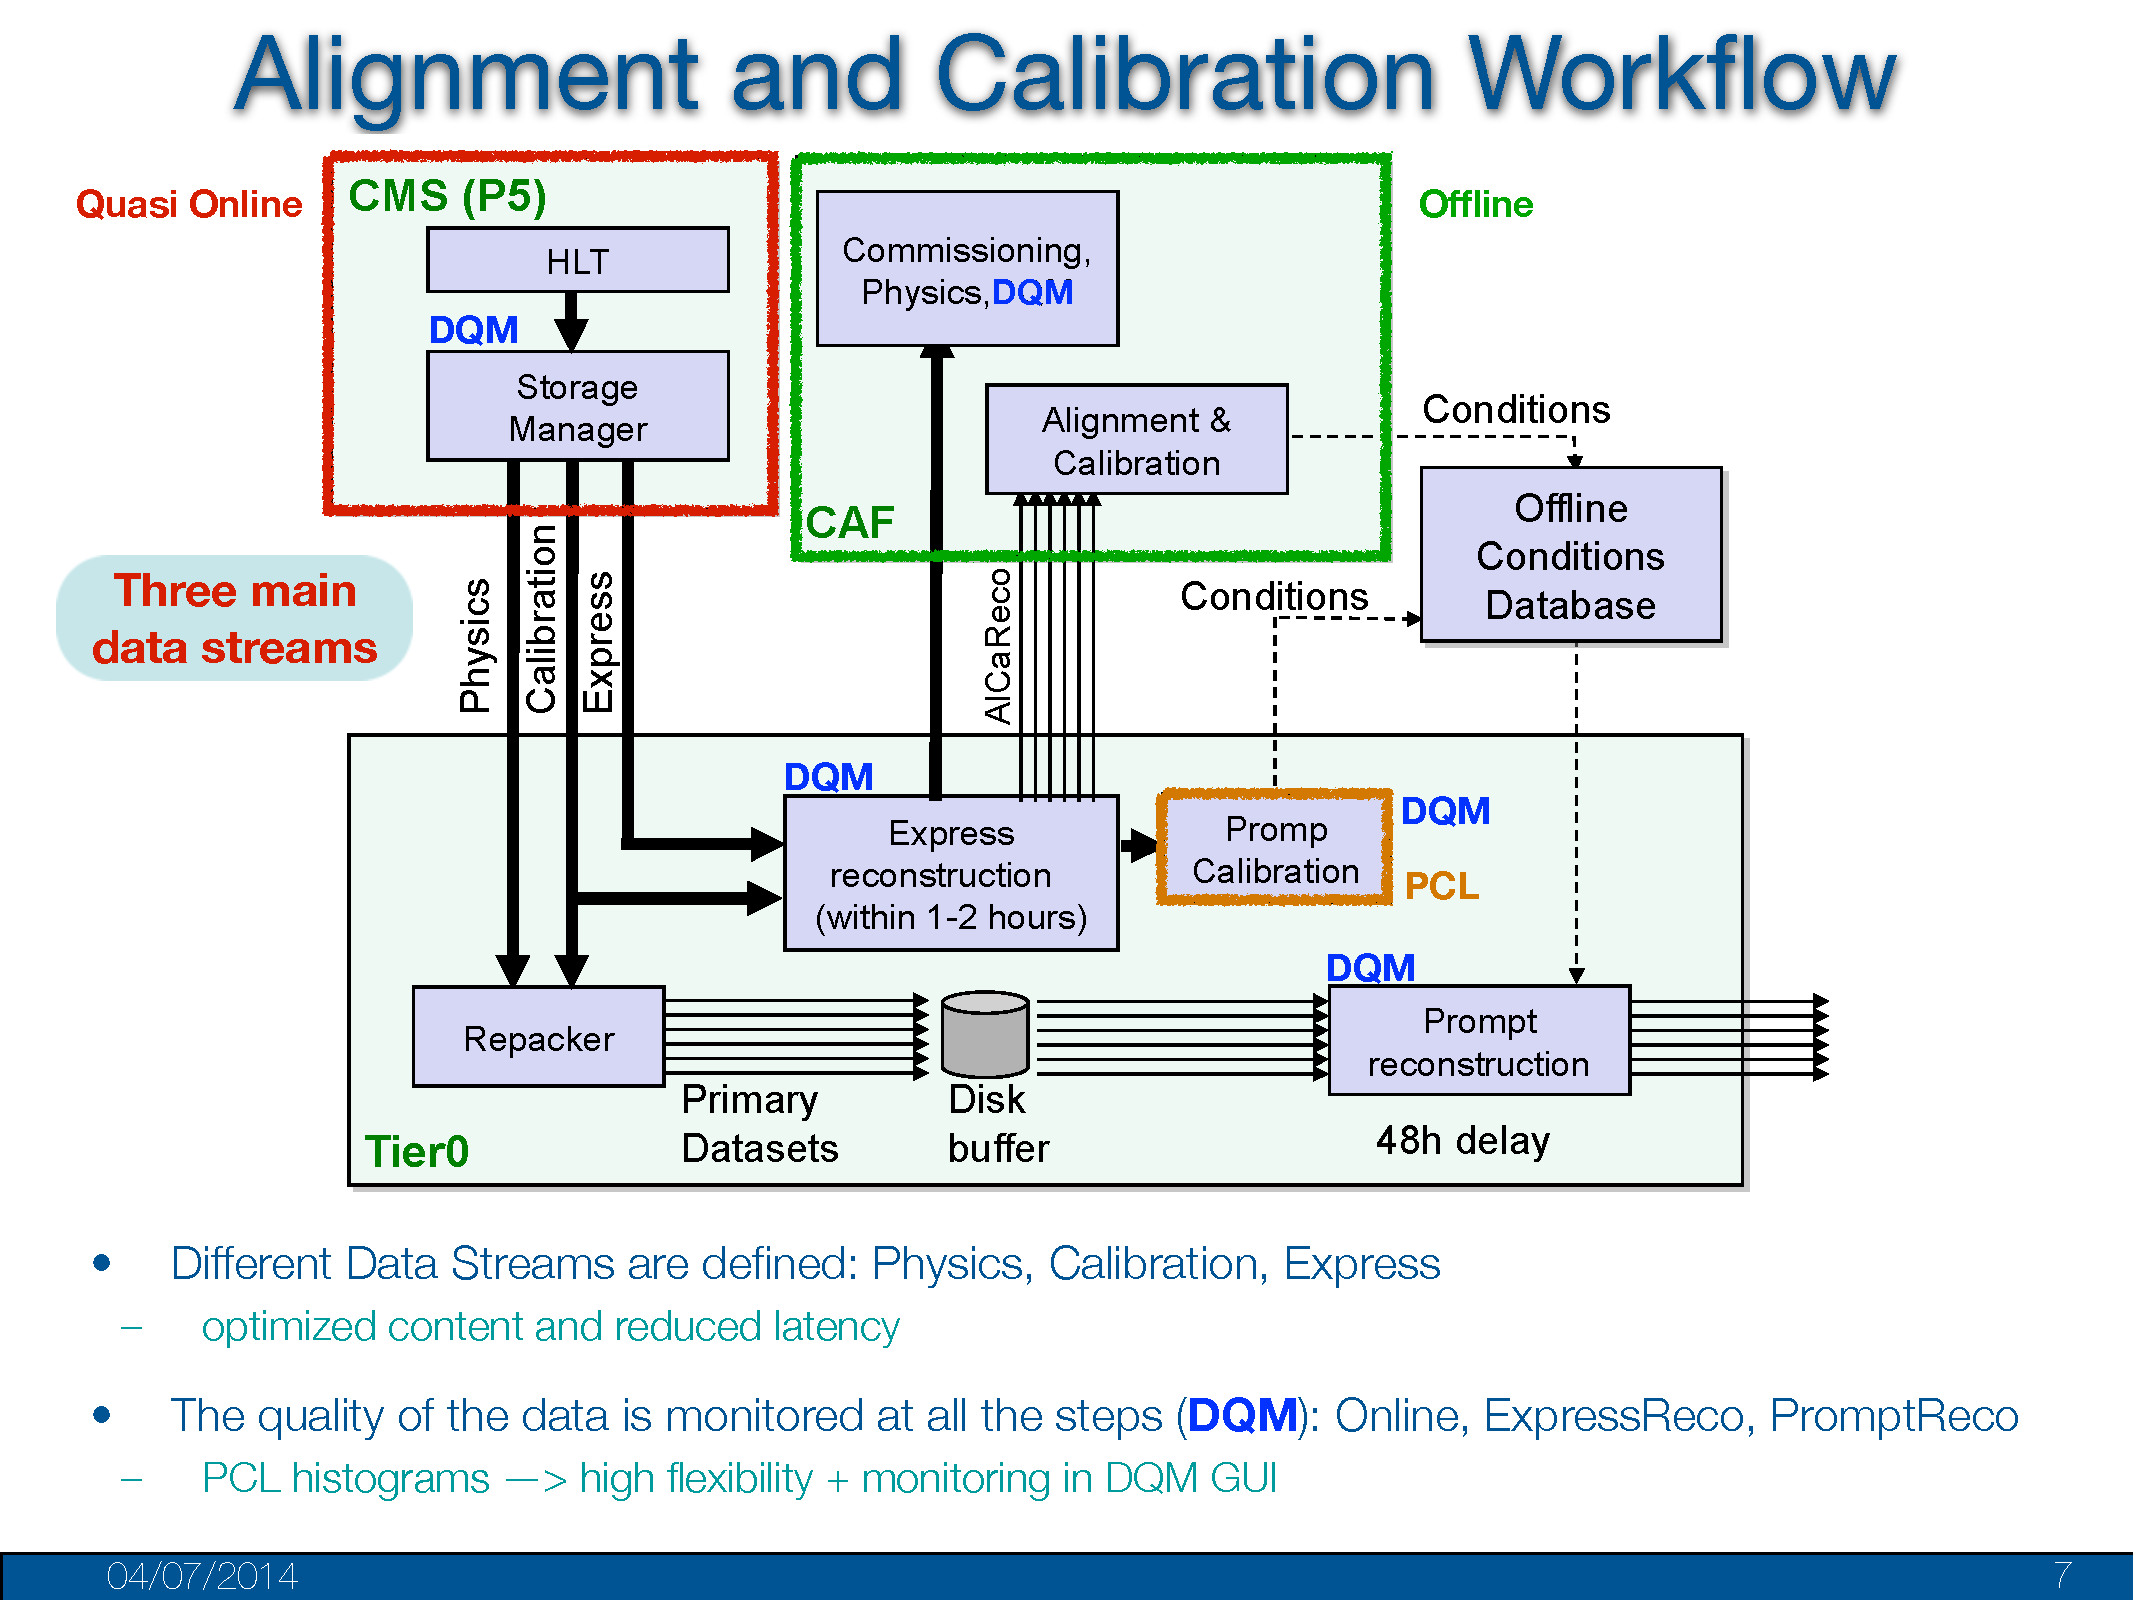
\includegraphics[width=.9\textwidth,clip=true,viewport=0 180 900 700]{figs/cms/AlCa.pdf}
\caption{Alignment and calibration data-processing flow.\label{fig:AlCa}}
\end{figure}
